\pagebreak
\checkoddpage
\ifodd\thepage
	\null
	\newpage
\fi

\setcounter{chapter}{3} % Manually set the chapter counter to 1
\setcounter{figure}{0}  % Reset the figure counter to 0
\thispagestyle{empty}

\begin{minipage}{\textwidth}
	\vspace{2.25cm}
	{%
		\centering
		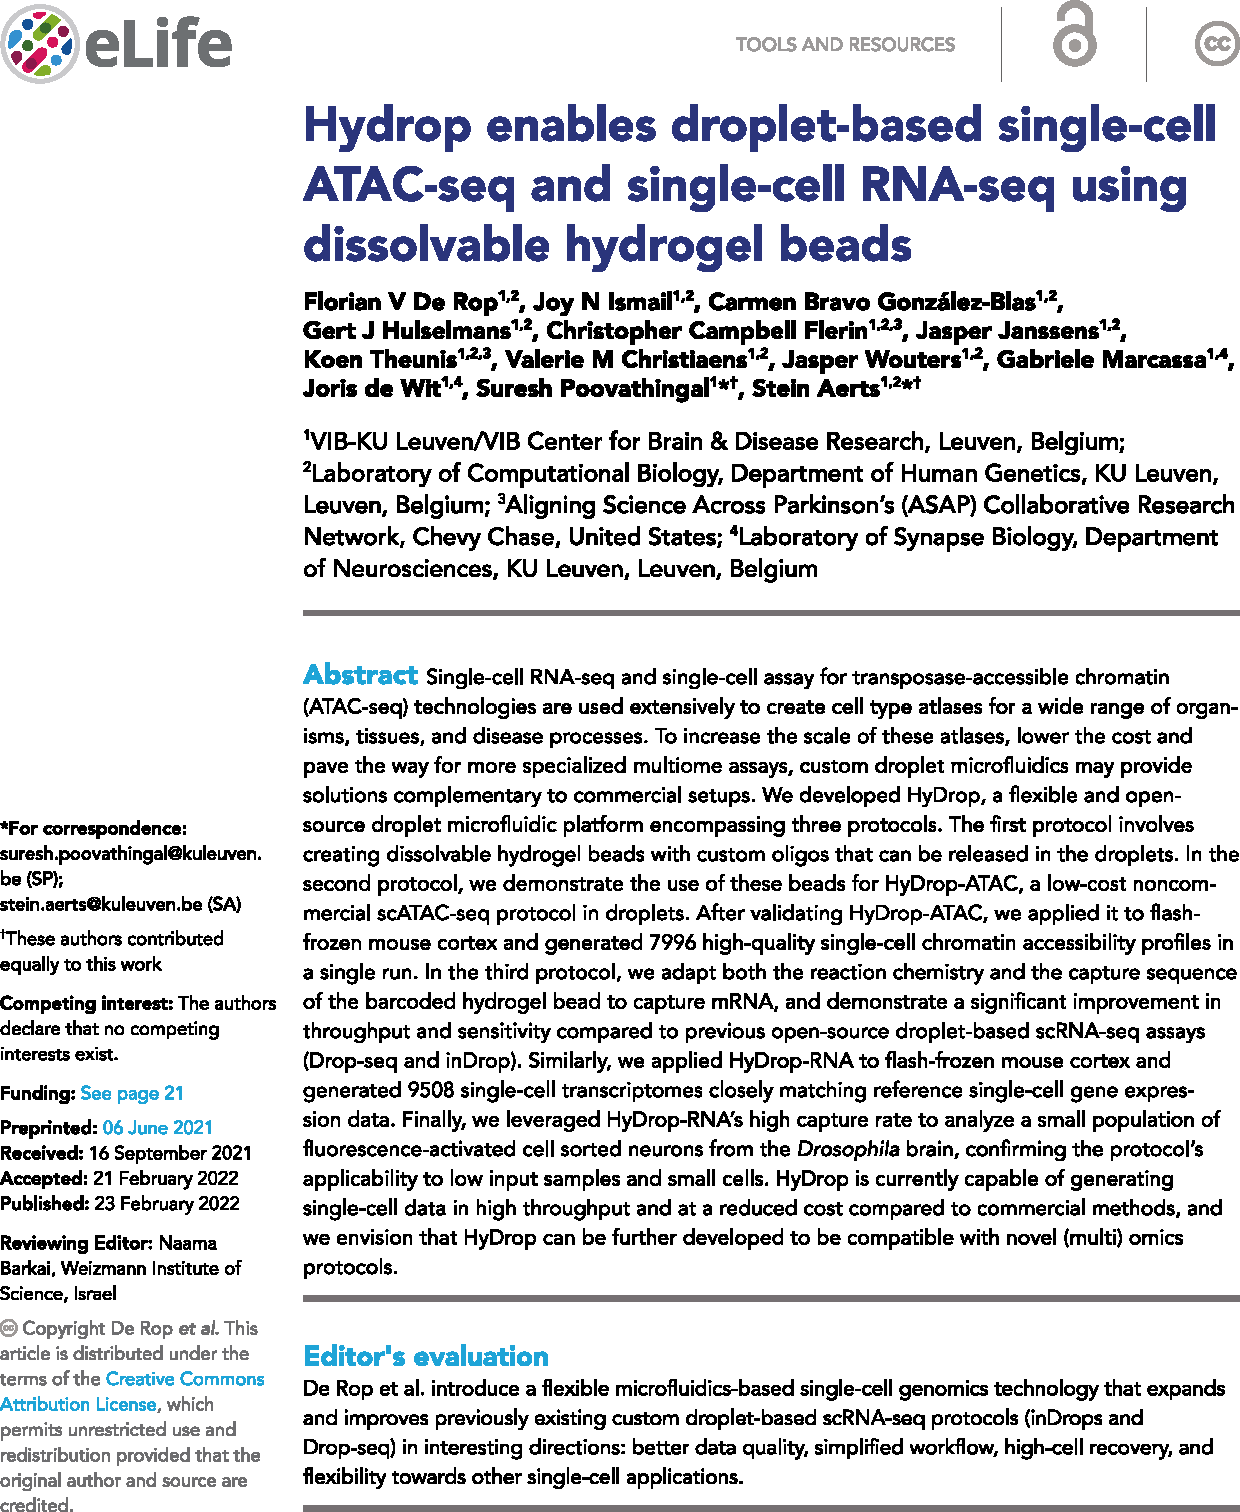
\includegraphics[width=\textwidth]{im/2021_elife_fixed.pdf}
		\captionsetup{width=0.80\linewidth}
		\vspace{0.5cm}
		\captionof{figure}[Article title page of "Hydrop enables droplet-based single-cell ATAC-seq and single-cell RNA-seq using dissolvable hydrogel beads"]{Article title page of "Hydrop enables droplet-based single-cell ATAC-seq and single-cell RNA-seq using dissolvable hydrogel beads" \notefullcite{derophydropenablesdropletbased2022}.}
		% \label{fig:sequencing_diagram_for_second_bead_design}
	}%
\end{minipage}

\setcounter{chapter}{2} % Manually set the chapter counter to 1

\chapter{Design and Development of HyDrop-ATAC and HyDrop-RNA}
\setcounter{figure}{1}  % Reset the figure counter to 0
In this chapter, we will walk through the design and development of HyDrop, our cost-efficient and transparent single-cell ATAC (and single-cell RNA) sequencing platform. We published this work in eLife in 2022\sjcitep[.]{derophydropenablesdropletbased2022}

\section{Motivation}
At the start of this project in 2018, single-cell sequencing methods had become established research tools but were still expensive and complicated enough to preclude routine use. At the time, academic scRNA-seq protocols were either low in throughput\sjcitep[,]{islamCharacterizationSinglecellTranscriptional2011, ramskoldFulllengthMRNASeqSinglecell2012, hashimshonyCELSeqSinglecellRNASeq2012, sasagawa2013quartz} or low in sensitivity\sjcitep[,]{macoskohighlyparallelgenomewide2015, gierahnSeqWellPortableLowcost2017, caoComprehensiveSinglecellTranscriptional2017,kleinDropletBarcodingSinglecell2015} and reserved for use by specialised labs. The majority of single-cell experiments were performed using the 10x Chromium, a commercial solution offered by 10x Genomics which packaged inDrop's droplet microfluidic cell isolation with aspects of SMART-seq's RNA library preparation into a user-friendly kit. This kit provided a reliable - and more importantly \textit{convenient} - way to generate high-quality single-cell RNA-seq libraries\sjcitep[]{mereuBenchmarkingSinglecellRNAsequencing2020}. Many researchers preferred to use this kit, since it struck a comfortable balance between throughput and sensitivity per money spent.

We made three observations:
\begin{enumerate}[noitemsep]
	\item At a cost of ~\euro{\num{10000}} per 8 samples of 10 000 cells, exploratory use of the 10x scRNA kit was still impractical.
	\item The kit operated as a black box, with limited possibility for modification.
	\item The kit's sensitivity was around 10 times higher than inDrop and Drop-seq's, implying that the sensitivity ceiling for droplet-based methods had not yet been reached by open-source methods.
\end{enumerate}

In addition, a droplet-based single-cell ATAC sequencing method was not available yet, constraining researchers to either low-sensitivity\sjcitep[]{cusanovichMultiplexSinglecellProfiling2015} or low-throughput\sjcitep[]{buenrostroSinglecellChromatinAccessibility2015,chenRapidRobustMethod2018} methods. Since droplet methods had provided a balanced trade-off between throughput and sensitivity that fit our lab's needs\sjcitep[]{davie2018single}, we set out to develop such a method. Finally, we also understood that combined scRNA/ATAC-seq would be necessary in future studies to deconvolve the individual and (cross-) combined effects of gene expression and chromatin accessibility. A better understanding of how to design and build a droplet-based scATAC-seq method would be a good stepping stone to building multiomics technologies. These circumstances prompted us to start development of our own droplet-based sequencing method. Specifically, we wanted to build an open-source platform capable of both scRNA-seq and scATAC-seq, at higher sensitivities than inDrop and Drop-seq. This project had already been initiated before my arrival at the lab, and I spent my first year as a master thesis student continuing this development.

\section{Design and main technical challenges}
% Besides speed, throughput and reduction in reagent cost, droplet microfluidics provide another key advantage: when cells are physically isolated from one another in droplets, we can fully lyse each cell akin to what happens in a microwell-based experiment. A drawback is that cells cannot be easily washed or accessed anymore after once encapsulated, precluding more complex protocols. The next step in the single-cell indexing process is the introduction of the cell barcode oligonucleotide.

One of the first design choices was whether we should use inDrop or Drop-seq style beads. Drop-seq's beads are made out of solid resin surface-coated with oligonucleotides whereas inDrop uses a soft, deformable polyacrylamide hydrogel with oligonucleotide barcodes loaded throughout. Both ideas are similar on the surface, but inDrop's soft hydrogel beads have one major advantage: they can be densely stacked in a microfluidic channel, leading to deterministic loading. This enables a higher cell capture rate of > 80\% versus < 5\% (see also \autoref{sect:single_cell_sequencing_tech}). We also considered that manufacturing and barcoding polyacrylamide hydrogels would be more straightforward than resin beads, which we would need to source from commercial suppliers.

Both inDrop and Drop-seq's approaches face diffusion-related limitations: in Drop-seq, RNA transcripts need to diffuse from the cell onto the surface of the bead, whereas in inDrop, barcode oligonucleotides need to diffuse from the center of the polyacrylamide bead into the bulk of the reaction. We hypothesised that volumetric oligonucleotide loading and release might outperform a surface-constrained process.

% \begin{figure}[h]
% 	\centering
% 	\includegraphics[width=0.85\linewidth,height=5cm]{example-image-a}
% 	\caption[inDrop \& Drop-seq diffusion limits]{inDrop \& Drop-seq diffusion limits}
% \end{figure}

Next, we considered the bead barcoding reaction. In Drop-seq, oligonucleotide barcodes are synthesized directly on the resin bead in 4\textsuperscript{12}. In inDrop, oligonucleotide sub-barcodes are annealed and copied to a primer stub by linear extension in 96\textsuperscript{3} split-pooling. We considered that linear amplification rather than isothermal extension could lead to higher bead barcoding reaction efficiency, subsequent higher density of barcodes within the bead, and higher in-droplet target capture as a result.

We also wanted to replace inDrop's photocleavable oligonucleotide linker by a disulfide bond, permitting the release of barcodes by reduction with DTT. This change would remove inDrop's requirement to work in the dark and possibly increase sensitivity. After all, ambient light exposure to light could cause the beads to prematurely release their barcodes - reducing the assay's specificity. (see \notefullcite{deropOptimisationInDropScRNAseq2019} for more details). By the end of the year, we had accomplished the following:

\begin{enumerate}[noitemsep]
	\item We designed and manufactured a microfluidic chip for the generation of the stable acrylamide monomer emulsions needed to produce polyacrylamide hydrogel beads using soft lithography\sjcitep[.]{xiaSoftLithography1998} We characterised the relationship between oil and water flow rates on this chip, and predicted flow rates that would generate \SI{50}{\micro\metre} diameter droplets with minimal size variance using iterative linear model optimisation (\autoref{fig:bead_diameter_optimisation}). The resulting beads were indeed of a stable \SI{53}{\micro\metre} diameter with a standard deviation of \SI{5}{\micro\metre}.

	      \svgfigure{im/indrop_model.pdf_tex}
	      {Bead diameter optimisation}
	      {Bead diameter optimisation strategy. From \notefullcite{deropOptimisationInDropScRNAseq2019}.}
	      {fig:bead_diameter_optimisation}

	\item We barcoded the resulting \SI{53}{\micro\metre} polyacrylamide hydrogel beads using inDrop's split-pool protocol, producing 96 \texttimes 96 \texttimes 96 possible cell barcodes across all beads (\autoref{fig:preliminary_barcoding_split_pool_design}). Importantly, the photocleavable linker was replaced by a disulfide bond as mentioned previously.

	\item We designed a new cell encapsulation microfluidic chip which included several layers of passive filters due to prior experiences with flow-obstructing dust particles. Using this updated design, we were able to reliably encapsulate single cells with reagent mixes across several experiments.

	      \svgfigure{im/indrop_chip_zoom.pdf_tex}
	      {Droplet encapsulation chip design}
	      {Droplet encapsulation chip design. Reproduced from \notefullcite{deropOptimisationInDropScRNAseq2019}.}
	      {fig:indrop_chip_zoom}

	\item To implement scRNA-seq on our now functional droplet platform, we tested several different cDNA generation and subsequent sequencing library preparation strategies. We ultimately settled on a protocol that was based on in-droplet Maxima H Minus reverse transcription, PCR amplification of cDNA by KAPA polymerase, and NEB Next Ultra II FS DNA sequencing library preparation. This protocol was different from both inDrop, which uses a more involved reverse transcription \textrightarrow second-strand synthesis \textrightarrow in-vitro transcription \textrightarrow random hexamer reverse transcription \textrightarrow PCR workflow, and Drop-seq, which relies on Tn5-based sequencing library prep from cDNA.
\end{enumerate}

In short, we had set up a workflow for producing hydrogel beads, barcoding those beads using linear amplification, and using those in scRNA-seq experiments that produced sequenceable libraries. In parallel to the scRNA-seq research, we began began preliminary scATAC-seq trials. This required the production of a new type of beads, this time with oligos that annealed to the Tn5 insertion adapter sequence instead of to poly(A) tails. Our scATAC-seq protocol relied on encapsulating pre-tagmented single nuclei into droplets together with the new ATAC-seq compatible beads and a variety of polymerases and commercial PCR master mixes. PCR cycling these emulsions should then lead to pre-amplified scATAC-seq libraries. What followed was a long series of trial and error where we troubleshot a number of issues, often shared between the scRNA-seq and scATAC-seq protocols. In rough chronological order, we dealt with the following issues and optimisations:

\textbf{Problem:} While the bulk characteristics of our earliest scRNA-seq libraries were very promising (expected cDNA and final library fragment size distributions, 3' enriched as designed, decent alignment to reference transcriptome of \textasciitilde{40}\%), we were not able to sequence barcodes fully at first. Between 67\% and 70\% of the barcode reads contained poly-G repeats. Out of the remaining ~30\%, only 0.2\% matched our barcode whitelist, compared to the > 95\% expected for 10x Genomics scRNA-seq datasets. This failure made it impossible to assign transcripts to cell of origin.

\textbf{Solution:} At first, we thought that the custom sequencing primer used to sequence the cell barcodes might be at fault. We knew that our NextSeq500 used Illumina's 2-channel laser technology. G bases are encoded by the absence of signal, whereas the other three bases are encoded by positive fluorescence in either or both of the two dyes used. Poly-G base calls in the final data could thus be interpreted as the absence of any signal from the sequenced molecule, indicating that the sequencing primer may not have annealed properly - precluding the generation of any signal. We attempted to test this hypothesis by making a batch of mock beads in which the custom priming site was replaced by Illumina's standard primers - which are highly optimized for specificity. The resulting dataset yielded barcode reads of which now only 33\% had a poly-G problem, but still only around 23\% matched the whitelist - still far below what was necessary to do a successful single-cell sequencing experiment. Next, we redesigned the barcode structure so that the cell barcode was now read in one go, and did not require the use of a custom sequencing primer (\autoref{fig:sequencing_diagram_for_second_bead_design}). More than 90\% of the new barcode reads matched our whitelist. The remaining 10\% could be attributed to incorporation errors during vendor oligonucleotide synthesis, PCR, and sequencing errors.

Later on, this change also had an important effect on our scATAC-seq assay: it allowed us to sequence both ends of the chromatin fragments as opposed to only a single end. Since ATAC-seq quantifies Tn5 insertion events, this increases the counting sensitivity and positional accuracy of called peaks. Note that insertion events within the same enhancer are correlated due to proximity, so total count information content is not doubled. Finally, paired-end information also improves cross-contamination estimation: when two cell barcodes are statistically enriched in identical fragments (exact same insertion sites with base-pair accuracy), they are highly likely to be cross-contaminated\sjcitep[.]{lareau2020inference}

\textbf{Problem:} Our first generation of beads had its barcode oligo payload dispersed and linked to the the bead's hydrogel matrix using a cleavable disulfide linker. We hypothesized that diffusion of barcodes from the center of the polyacrylamide hydrogel bead into the droplet would be a slow and reaction rate-limiting process. To test diffusion, we measured the beads' total primer content before and after DTT incubation, using probe fluorescence as a proxy. A strong residual fluorescent signal after even 50 minutes of continuous incubation with 50 mM DTT confirmed that much of the initial primer population was retained within the bead. Since DTT has a molecular weight comparable to a single nucleotide, and has good water solubility, we did not expect its diffusion to be the rate-limiting factor.

\textbf{Solution:} We included N,N'-Bis(acryloyl)cystamine (BAC) in the hydrogel polymerisation reaction, replacing classic bisacrylamide and making the gel polymer's crosslinks reversibly cleavable under reducing conditions. These beads dissolved in under 10 minutes of exposure to 10 mM DTT at room temperature.

\textbf{Problem:} Cell-in-oil emulsions did not survive PCR thermocycling, which was necessary for amplifying accessible genome fragments in ATAC-seq. Microdroplets coalesced into large oil drops, meaning that bulk rather than single-cell libraries would be generated.

\textbf{Solution:} We tested various changes to the protocol, including different PCR master mixes (NEB, KAPA, Terra, Q5), PCR programs (number of cycles, temperatures) and density regulators (PEG-8000, Iodoxanol), but this issue was ultimately solved as a welcome side-effect of making the beads dissolvable. We then realised that the thermocycling induced convective flows in the emulsions, leading to bead collisions which resulted in emulsion breaking. When the beads were dissolved within the droplets, this effect disappeared and emulsions remained stable throughout PCR cycling.

We were now able to sequence cell barcodes, align them to a whitelist, align the genomic reads to a reference (both transcriptomic and genomic), and keep stable emulsions throughout the process. Our scRNA-seq data was 3' transcriptome enriched, and our scATAC-seq data aggregated into peaks and exhibited typical ATAC-seq fragment length distribution, with nucleosome and helical pitch. However, data in both our scATAC-seq and scRNA-seq libraries did not aggregate into pure cells in mixed-species experiments: all "cells" contained a mixture of human and mouse reads. This problem also manifested during cell filtration: rather than sharp cutoffs between cell barcodes and low-signal noise barcodes, we had a gradual transition from cell to noise. This would prove to be the most challenging issue during the entire HyDrop research campaign.

This idea was strongly supported by evidence in Sanger sequencing, where we observe that the first sub-barcode locus is very pure, but the middle sub-barcode locus is not, and the third sub-barcode locus is pure again. This could be explained by [[x]].

\textbf{Solution:} One of the first things we changed was introducing extra primer purifications after emulsion breaking. We had noticed that at this stage, even after a magnetic bead purification, our libraries still had extreme enrichment of barcode primers.

This mechanism of contamination could explain both observations that convinced us that our method was not single-cell: the vague separation between true cells and background noise barcodes on the kneeplot could be caused by all unused barcodes associating with transcripts/fragments post-emulsion breaking, and the lack of cell types could be explained by the dilution of each single-cell profile with random transcripts/fragments due to barcode promiscuity

We reasoned that these primers would carry over into downstream PCR amplification, where they could randomly capture un-tagged mRNA or ATAC fragments, or even out-compete PCR primers annealing to correctly barcoded DNA molecules. Adding a second bead wash strongly reduced this peak, but only mildly improved the species mixing we observed in our libraries. For scATAC-seq, we also tried using exponential in-droplet PCR by adding a reverse primer to the reaction, hoping to improve barcode consumption at the risk of introducing PCR biases, but this did not improve purity.

\textbf{Problem:} Thus far, we had not yet confirmed that our PCR-produced beads were pure: cross-contamination could occur during bead production, leading to mixed-barcode beads which generate random noise downstream. Cross-contamination of sub-barcode primers could be amplified throughout the PCR bead barcoding procedure. In order to test this, we reduced the three rounds of sub-barcoding (96\textsuperscript{3} split-pooling) to two rounds (384\textsuperscript{2}). This change improved species purity in our species-mixing experiments, but still not to usable levels.

\textbf{Solution:} Finally, we reduced the acrydite primer load during bead generation from \SI{50}{\micro\molar} to \num{1.5}, \num{6}, \num{12.5} and \SI{6.25}{\micro\molar}, drastically reducing the total number of available sites for barcoding. Beads made with the 6 and \SI{12.5}{\micro\molar} primer concentrations immediately produced species-pure scRNA-seq, and later scATAC-seq libraries, whereas the \SI{1.5}{\micro\molar} condition did not produce detectable cDNA. Most likely, this change affected purity in two ways: first, the polymerase reaction is now more likely to saturate the number of available barcode sites, reducing the number of available "previous-round" priming sites in the next round. Second, a lower total primer load released into the droplet is more likely to be purified out completely. Later research (post-publication) also indicated that washing bead wells individually during barcoding rather than in a pooled manner further increased bead purity and thus sensitivity. Individual dilutive washing of the sub-barcoding primers before pooling prevents these barcodes from annealing with remaining un-templated sites from the previous round of barcoding, improving barcode purity.

At this point, we were certain we had functional scRNA-seq and scATAC-seq working with our beads and library preparation workflows. Mixed-species experiments returned pure (\textasciitilde{90}\%) single-cell profiles, and we were able to assign cell types to our first experiments on \textit{Drosophila} and mixed-cancer cell lines. In parallel we had also implemented a number of small novelties. For example, addition of Pitstop 2, a selective clathrin-mediated endocytosis inhibitor which also permeabilizes the nuclear membrane by destabilizing nucleoporin complexes, to the tagmentation reaction was known to improve Tn5 diffusion into the nucleus\sjcitep[.]{mulqueen2020improved} We also added guanidinium isothiocyanate, a strong chaotrope known to denature proteins and solubilize nucleic acids, to the emulsion after PCR. Both additions led to slight library yield improvements. We also titrated several different sources of Tn5 and found no discernible difference in performance or fragment biases between commercial (Illumina, diagenode) and open-source Tn5\sjcitep[.]{picellitn5transposasetagmentation2014} Since Nextera Tn5 comprises 46\% of the droplet reaction cost, savings made by using in-house Tn5 are considerable.

In addition, we tested a number of optimisations for HyDrop-RNA. Exonuclease I (Exo I) has been used in single-cell RNA-seq workflows to remove excess primers and barcodes that could lead to non-specific priming\sjcitep[.]{macoskohighlyparallelgenomewide2015} Addition or exclusion of Exo I did not appear to make a difference in sensitivity. Introduction of two riboguanosines in the template-switching oligo, which improve thermal annealing stability to 3' \verb|CCC| motif of the untemplated cDNA, also did not appear to increase sensitivity[.]{picellifulllengthrnaseqsingle2014} Second-strand synthesis through Bst2.0 or Klenow fragment\sjcitep[]{stickels2020highly} showed improvements, but the best cDNA amplification strategy was PCR thermocycling supplemented with GTP\sjcitep[.]{hagemannjensensinglecellrnacounting2020}

soft lithography paper

\section{Conclusion}